\documentclass[12pt,a4paper]{article}
\usepackage[utf8]{inputenc}
\usepackage[french]{babel}
\usepackage{geometry}
\usepackage{hyperref}
\usepackage{listings}
\geometry{margin=2.5cm}
\usepackage[T1]{fontenc}
\usepackage{lmodern}
\usepackage{amsfonts}
\usepackage{amssymb}
\usepackage{titlesec}
\usepackage{geometry}
\usepackage{tikz} % Pour les cadres et effets
\usepackage{geometry}
\geometry{margin=2.5cm}
\usepackage{fancyhdr}
\pagestyle{fancy}
\fancyhf{}
\rhead{TP2}
\lhead{Power BI}
\cfoot{\thepage}
\usepackage{graphicx}   % Pour insérer des images
\usepackage{listings}   % Pour afficher du code
\usepackage{xcolor}     % Pour la coloration syntaxique
\usepackage{caption}    % Pour les légendes personnalisées
\usepackage{float}      % Pour le placement des figures

\lstset{
	language=Java,
	basicstyle=\ttfamily\small,
	keywordstyle=\color{blue},
	commentstyle=\color{gray},
	stringstyle=\color{red},
	breaklines=true,
	frame=single,
	showstringspaces=false,
	numbers=left,
	numberstyle=\tiny\color{gray},
	inputencoding=utf8,
	extendedchars=true,
	literate=              % Gestion des accents
	{é}{{\'e}}1
	{è}{{\`e}}1
	{ê}{{\^e}}1
	{ë}{{\"e}}1
	{û}{{\^u}}1
	{ù}{{\`u}}1
	{â}{{\^a}}1
	{à}{{\`a}}1
	{î}{{^\i}}1
	{ô}{{\^o}}1
	{ç}{{\c c}}1
	{É}{{\'E}}1
	{È}{{\`E}}1
	{Ê}{{\^E}}1
	{À}{{\`A}}1
	{Â}{{\^A}}1
	{Î}{{\^I}}1
	{Ô}{{\^O}}1
	{Ç}{{\c C}}1
}

\geometry{hmargin=2.5cm,vmargin=2.5cm}

% Définition de la couleur bleu-gris
\definecolor{bluegray}{RGB}{200,220,240}
\begin{document}

% Page de garde
	\begin{titlepage}
		\centering
		
		% Logo de l'institut
		\textsc{\LARGE Institut National Supérieur\\[0.5cm] d'Informatique}\\[1.5cm]
		
		
\includegraphics[width=0.3\textwidth]{logo.jpg}\\[1cm]
		
		% Cadre avec bords arrondis et fond bleu-gris
		\vfill
		%%%%%%%%%%%%%%%%%%%%%
		\begin{center}
			\begin{tikzpicture}
				\node[rectangle,
				rounded corners=15pt,
				inner sep=15pt,
				fill=bluegray,
				draw=blue!50!black,
				line width=1.5pt,
				text width=0.9\linewidth,  % Réduire légèrement la largeur
				align=center] (box) {
					\fontsize{20}{24}\selectfont\bfseries
					TP 2 -- Analyse conditionnelle des \\ commandes selon \\les statuts et la localisation\\[0.8em]
					
				};
			\end{tikzpicture}
		\end{center}
		%%%%%%%%%%%%%%%%%%%%%%
		\vfill
		
		\begin{flushleft}
			\large
			\begin{center}
				\textbf{Étudiante:} ANDRIATSIFERANA No Kanto Lorida\\
			\textbf{Niveau:} Master 1 \\
			\textbf{Spécialité:} I2AD\\
            \textbf{Matricule:} 65/MA \\
			\textbf{Année académique:} 2025-2026\\
			\textbf{Date de rendu :} 21 juin 2025
			\end{center}
			
		\end{flushleft}
	
	\end{titlepage}
	
	\newpage

    \section*{Objectif du TP}
    L'objectif de ce TP est de manipuler les donn\'ees de commande \`a l'aide de Power Query en appliquant des transformations telles que : changement de types, conditions logiques, filtres dynamiques, et enrichissement de colonnes. L'analyse vise \`a identifier les commandes r\'ecentes, les clients \`a suivre, et \`a cibler des produits sp\'ecifiques.


    \subsection*{\textbf{1 - \underline{Charger la feuille Sheet1}} }
    \textbf{Code M :}
    \begin{lstlisting}[language=]
    Source = Excel.Workbook(File.Contents
        ("C:\INSI\cours\Power_BI\Data_BI\
        Commandes_Export.xlsx"), null, true),

    Sheet1_Sheet = Source{[Item="Sheet1",Kind="Sheet"]}[Data]
    \end{lstlisting}
    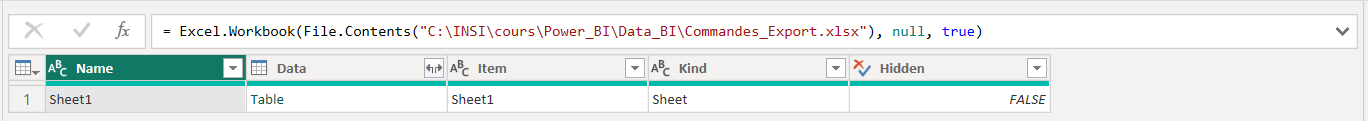
\includegraphics[width=\textwidth]{etape1.png}


     Les données brutes de \textbf{Sheet1} sont importées avec les en-têtes par défaut (ex : Colonne1, Colonne2...). Les entêtes ne sont pas clairs, cela rend les colonnes difficiles à exploiter.

    \subsection*{\textbf{2 - \underline{Promouvoir la premi\`ere ligne comme en-t\^ete}:}} 
    \textbf{Code M :}
    \begin{lstlisting}[language=]
    PromotedHeaders = Table.PromoteHeaders(Sheet1_Sheet, 
        [PromoteAllScalars=true])
    \end{lstlisting}
    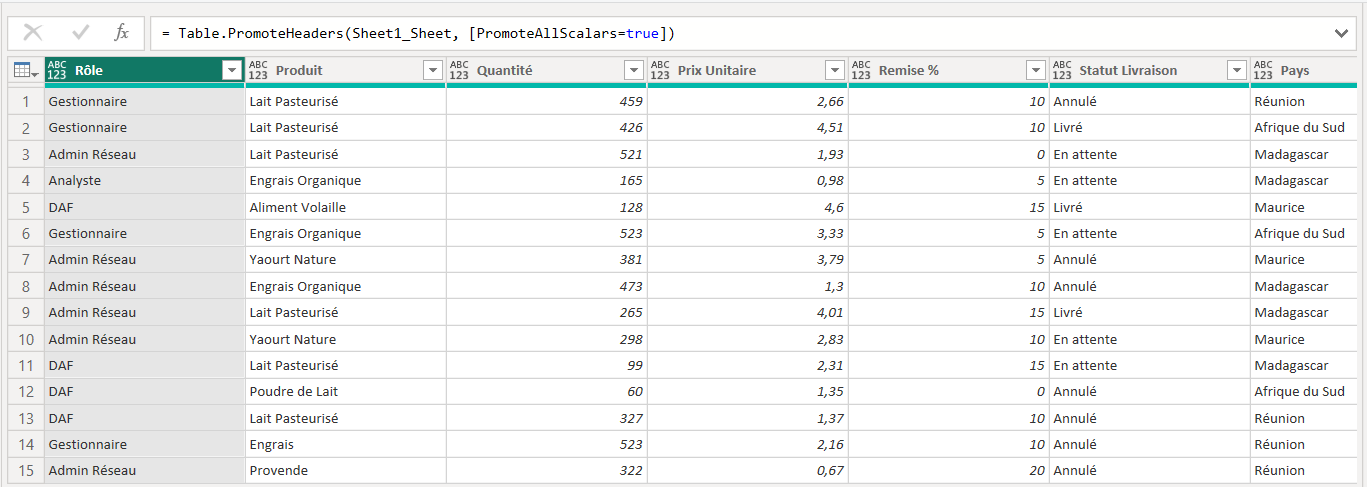
\includegraphics[width=\textwidth]{etape2.png}


    La premi\`ere ligne devient l'ent\^ete, ce qui permet de nommer correctement les colonnes. Les colonnes ont désormais des noms lisibles comme "Date Commande", "Produit", "Statut Livraison", ... Elle est essentielle pour appliquer des filtres ou des conditions logiques.


	\newpage
    
    \subsection*{3 - \textbf{\underline{Changer les types de colonnes}} }
    \textbf{Code M :}
    \begin{lstlisting}[language=]
    ChangedTypes = Table.TransformColumnTypes(PromotedHeaders, {
        {"Date Commande", type date}, 
        {"Quantit\'e", Int64.Type}, 
        {"Prix Unitaire", type number}
    })
    \end{lstlisting}

	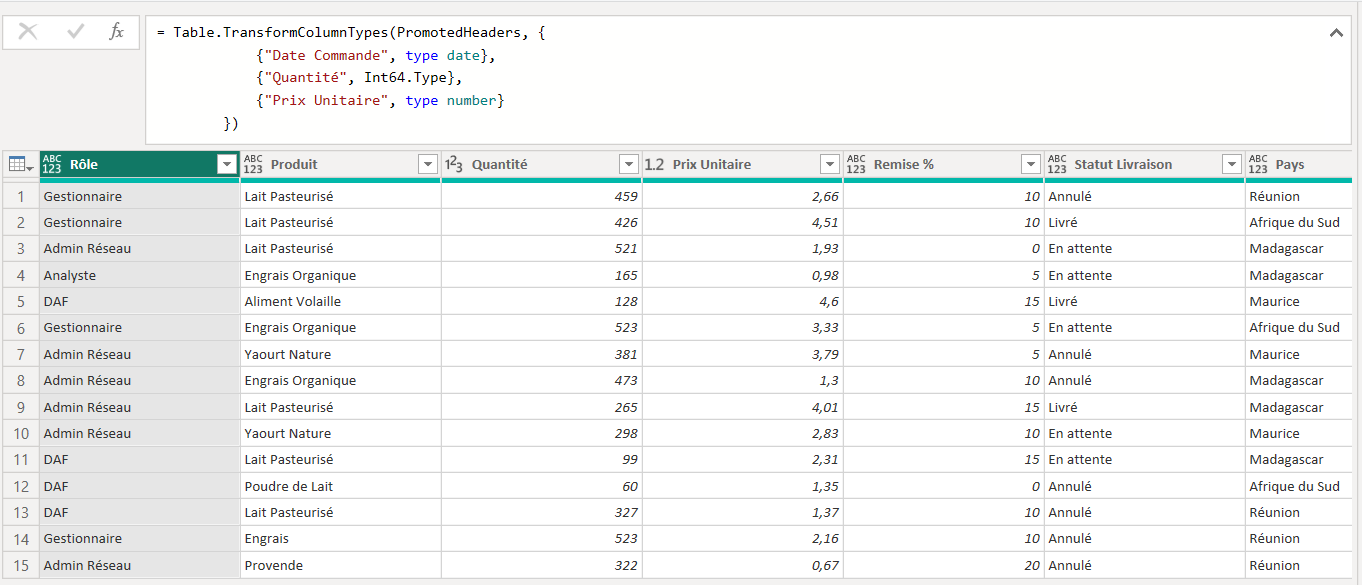
\includegraphics[width=\textwidth]{etape3.png}


     Les types sont modifi\'es pour garantir des op\'erations fiables sur les dates et valeurs num\'eriques. Ces conversions permettent à Power BI de traiter les données correctement, notamment pour effectuer des tris, des regroupements ou des calculs.

    

    \subsection*{4 - \textbf{\underline{Ajouter une colonne \og Commande R\'ecente\fg}}} 
    \textbf{Code M :}
    \begin{lstlisting}[language=]
    AjoutCommandeRecente = Table.AddColumn(ChangedTypes, "Commande R\'ecente", each if [Date Commande] > #date(2024, 1, 6) then "R\'ecente" else "Ancienne")
    \end{lstlisting}

	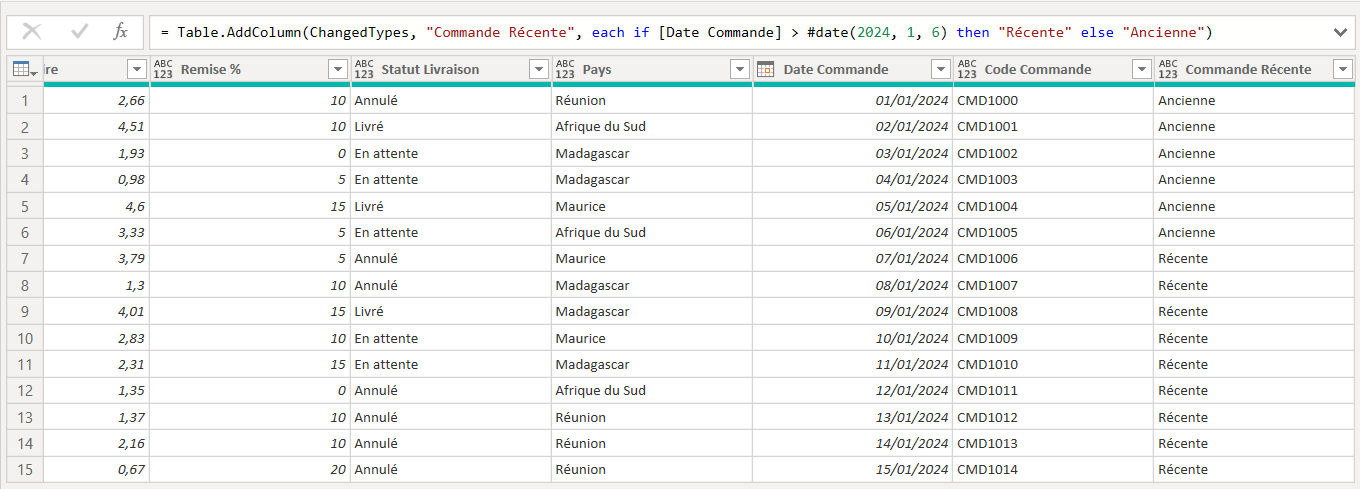
\includegraphics[width=\textwidth]{etape4.png}


     Une colonne indique "Récente" ou "Ancienne" selon la date de commande. On distingue rapidement les commandes récentes (après le 6 janvier 2024) des anciennes. Cela facilite les analyses temporelles.

	\newpage
    \subsection*{5 - \textbf{\underline{Ajouter une colonne \og Statut Client\fg}}} 
    \textbf{Code M :}
    \begin{lstlisting}[language=]
    AjoutStatutClient = Table.AddColumn(AjoutCommandeRecente, "Statut Client", each if [Statut Livraison] = "En attente" and [Pays] = "Madagascar" then "Client \`a suivre" else "Client r\'egulier")
    \end{lstlisting}

	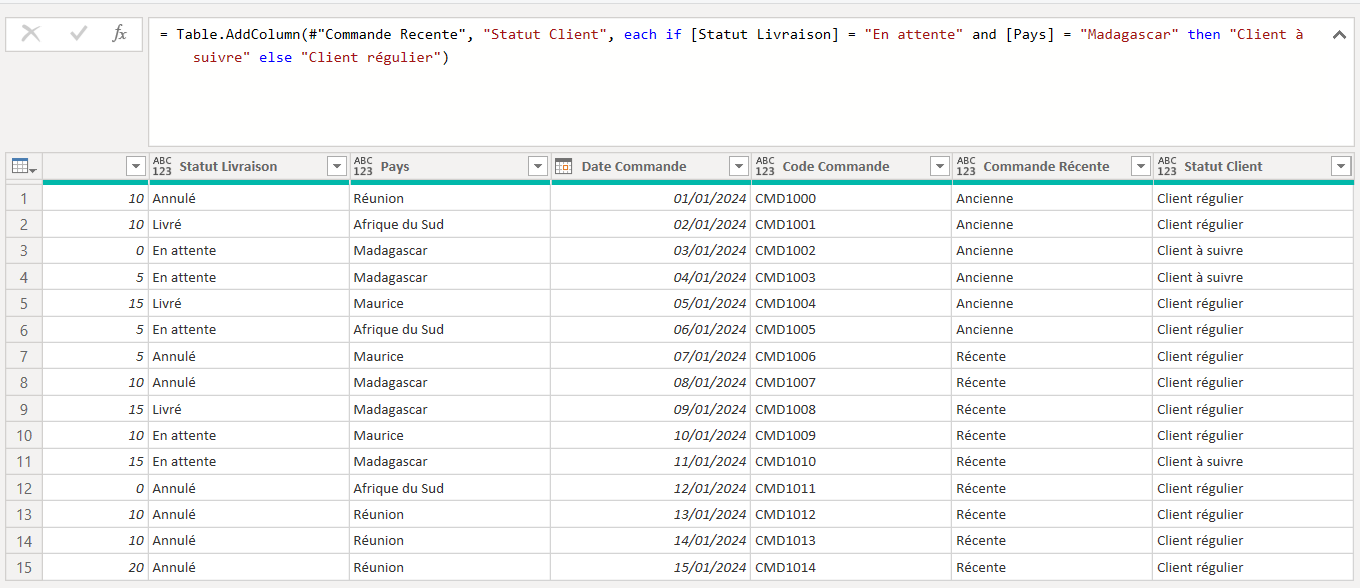
\includegraphics[width=\textwidth]{etape5.png}


    Une colonne indique "Client à suivre" si le client est à Madagascar et que la commande est "En attente", sinon "Client régulier". Cette étape identifie les clients potentiellement problématiques à surveiller, en croisant deux informations clés : le statut de livraison et la localisation.

    

    \subsection*{6 - \textbf{\underline{Filtrer les produits cibl\'es}}} 
    \textbf{Code M :}
    \begin{lstlisting}[language=]
    ProduitsFiltres = Table.SelectRows(AjoutStatutClient, each ([Produit] = "Lait Pasteuris\'e" or [Produit] = "Engrais Organique"))
    \end{lstlisting}

	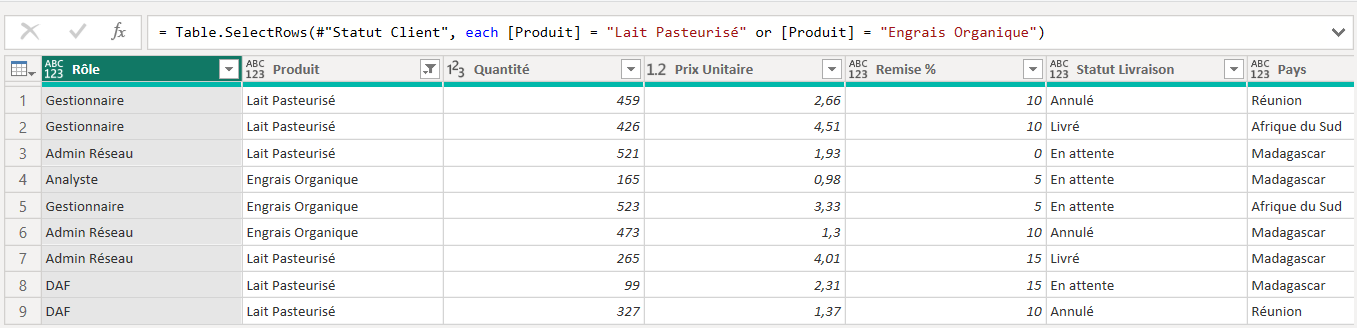
\includegraphics[width=\textwidth]{etape6.png}


     Seules les lignes contenant "Lait Pasteurisé" ou "Engrais Organique" sont conservées. On isole les produits d’intérêt pour cette analyse, ce qui rend les données plus ciblées et réduit le bruit.
	\newpage
    

    \subsection*{7 - \textbf{\underline{Supprimer les lignes \og Annul\'e\fg}}} 
    \textbf{Code M :}
    \begin{lstlisting}[language=]
    SansAnnule = Table.SelectRows(ProduitsFiltres, each [Statut Livraison] <> "Annul\'e")
    \end{lstlisting}

	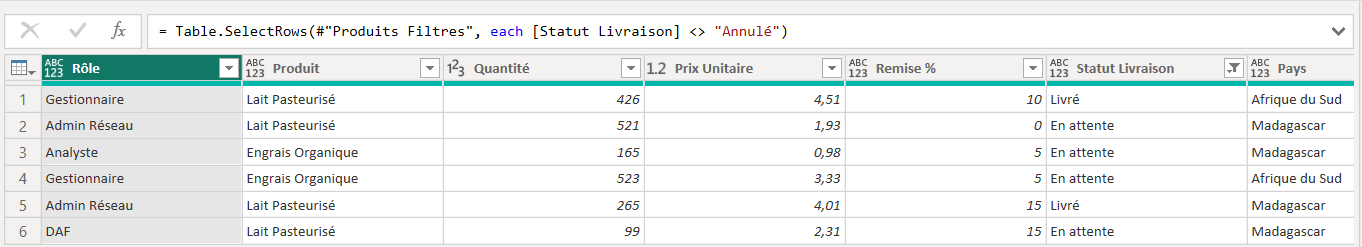
\includegraphics[width=\textwidth]{etape7.png}


     Les lignes avec "Statut Livraison = Annulé" disparaissent. Les commandes annulées ne doivent pas impacter l’analyse (pas de livraison ni de facturation), donc elles sont supprimées pour obtenir des données fiables.

    

    \subsection*{8 - \textbf{\underline{Trier par quantit\'e}}} 
    \textbf{Code M :}
    \begin{lstlisting}[language=]
    TrieParQuantite = Table.Sort(SansAnnule,{{"Quantit\'e", Order.Descending}})
    \end{lstlisting}

	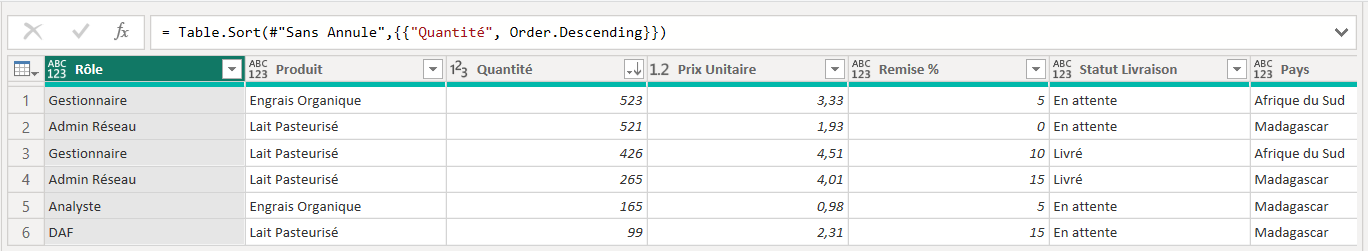
\includegraphics[width=\textwidth]{etape8.png}


     Les commandes sont classées du plus grand au plus petit en fonction de la quantité. Ce tri permet de repérer rapidement les commandes les plus importantes en volume, ce qui est utile pour la gestion de stock et la priorisation logistique.

    

    \section*{Conclusion}
    Ce TP a permis de ma\^itriser des transformations conditionnelles et logiques dans Power Query. Les colonnes ajout\'ees et les filtres appliqu\'es permettent une analyse cibl\'ee et op\'erationnelle, facilitant la prise de d\'ecision sur les clients \`a suivre et les produits prioritaires.

\end{document}
